\section{Handling Negative Weights in a BDT}\label{subsec:negWeights}
In section \ref{subsec:TraVal}, I mentioned the inclusion of sample weights in the training 
of the \ac{ML} models. Most weights are in the range of $w_i \in [0,1]$, but some sample weights are negative.
The negative weight problem is a well known problem in the world of \ac{ML}-analysis for \ac{HEP}, 
and is a consequence of higher perturbative accuracy. For the purpose of visualizing 
distributions and training a \ac{NN}, negative weights are not a problem. But, when using 
the weights in the training of the XGBoost classifier, the algorithm does not work\footnote{Upon further research 
in the codebase of XGBoost, it seems as though negative weights are not allowed as it interfere with XGBoost's use 
of the hessian matrix. Due to time constraints, I decided not to  pursue this further.}.  
\\
Before deciding how to mediate the issue, I decided to plot the distribution for 
a small subset of features for all the events with negative weights.
In figure \ref{fig:lep1_Pt_Neg} and \ref{fig:lep1_Phi_Neg} I plotted the distribution of the leading 
lepton for the features $P_t$ and $\phi$, but only including events with negative weights.
Additionally, I drew the distribution for the full data set for the same features in figures \ref{fig:lep1_Pt_nNeg}
and \ref{fig:lep1_Phi_nNeg}. By comparing the distributions, we can observe that the full data set and the 
negative weights' subset are very similar. There are differences in distributions when comparing the \ac{SM} 
individually, but when studying the background as a whole, the two sets exhibit the same trend across all 
regions. This means that the negative weights essentially scale the background uniformly over the full feature 
space, which motivates treating the negative weight problem uniformly over the full feature space.
\begin{figure}
    \makebox[0.95\linewidth][c]{%
    \centering
    \begin{subfigure}{.525\textwidth}
        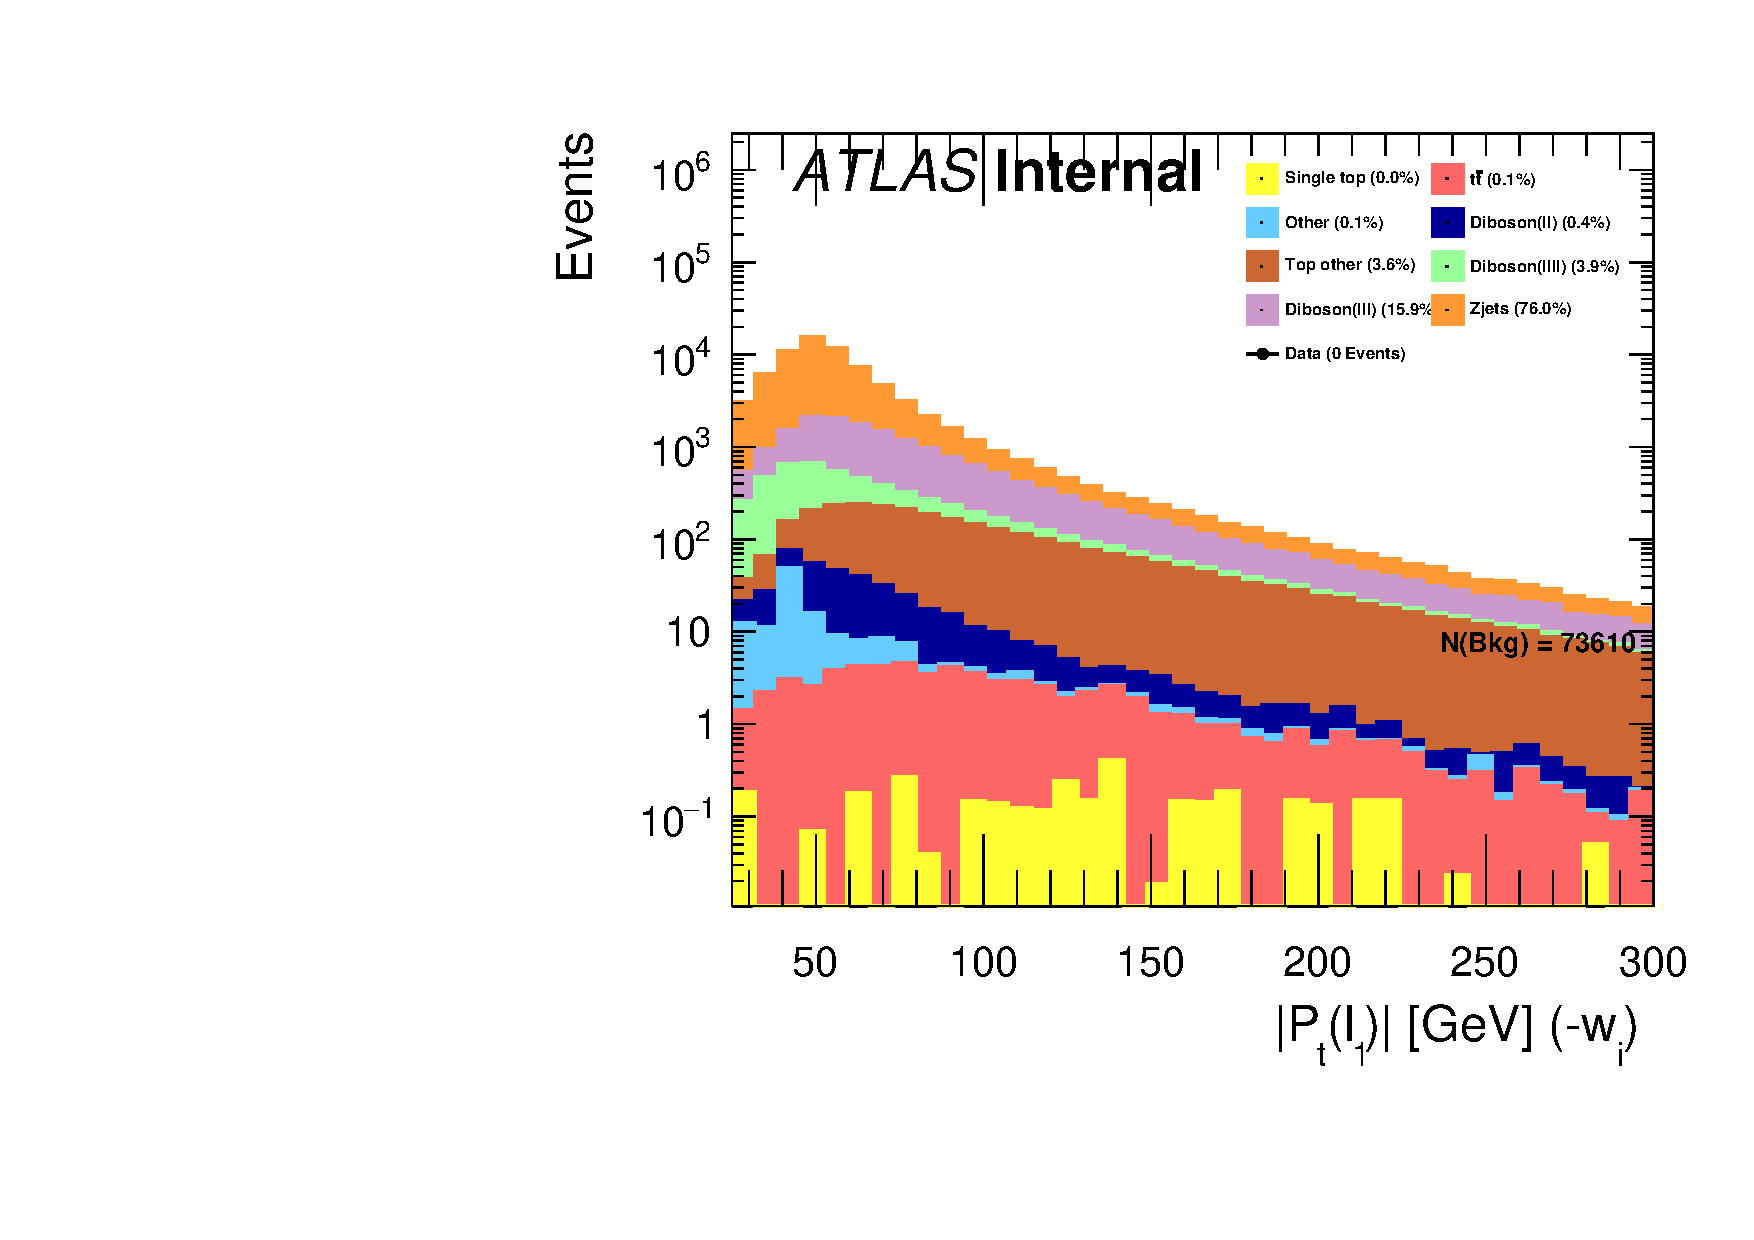
\includegraphics[width=\textwidth]{Figures/FeaturesHistograms/lep1_Pt_Neg.pdf}
        \vspace{-.75cm}
        \caption{}
        \label{fig:lep1_Pt_Neg}
    \end{subfigure}
    \begin{subfigure}{.525\textwidth}
        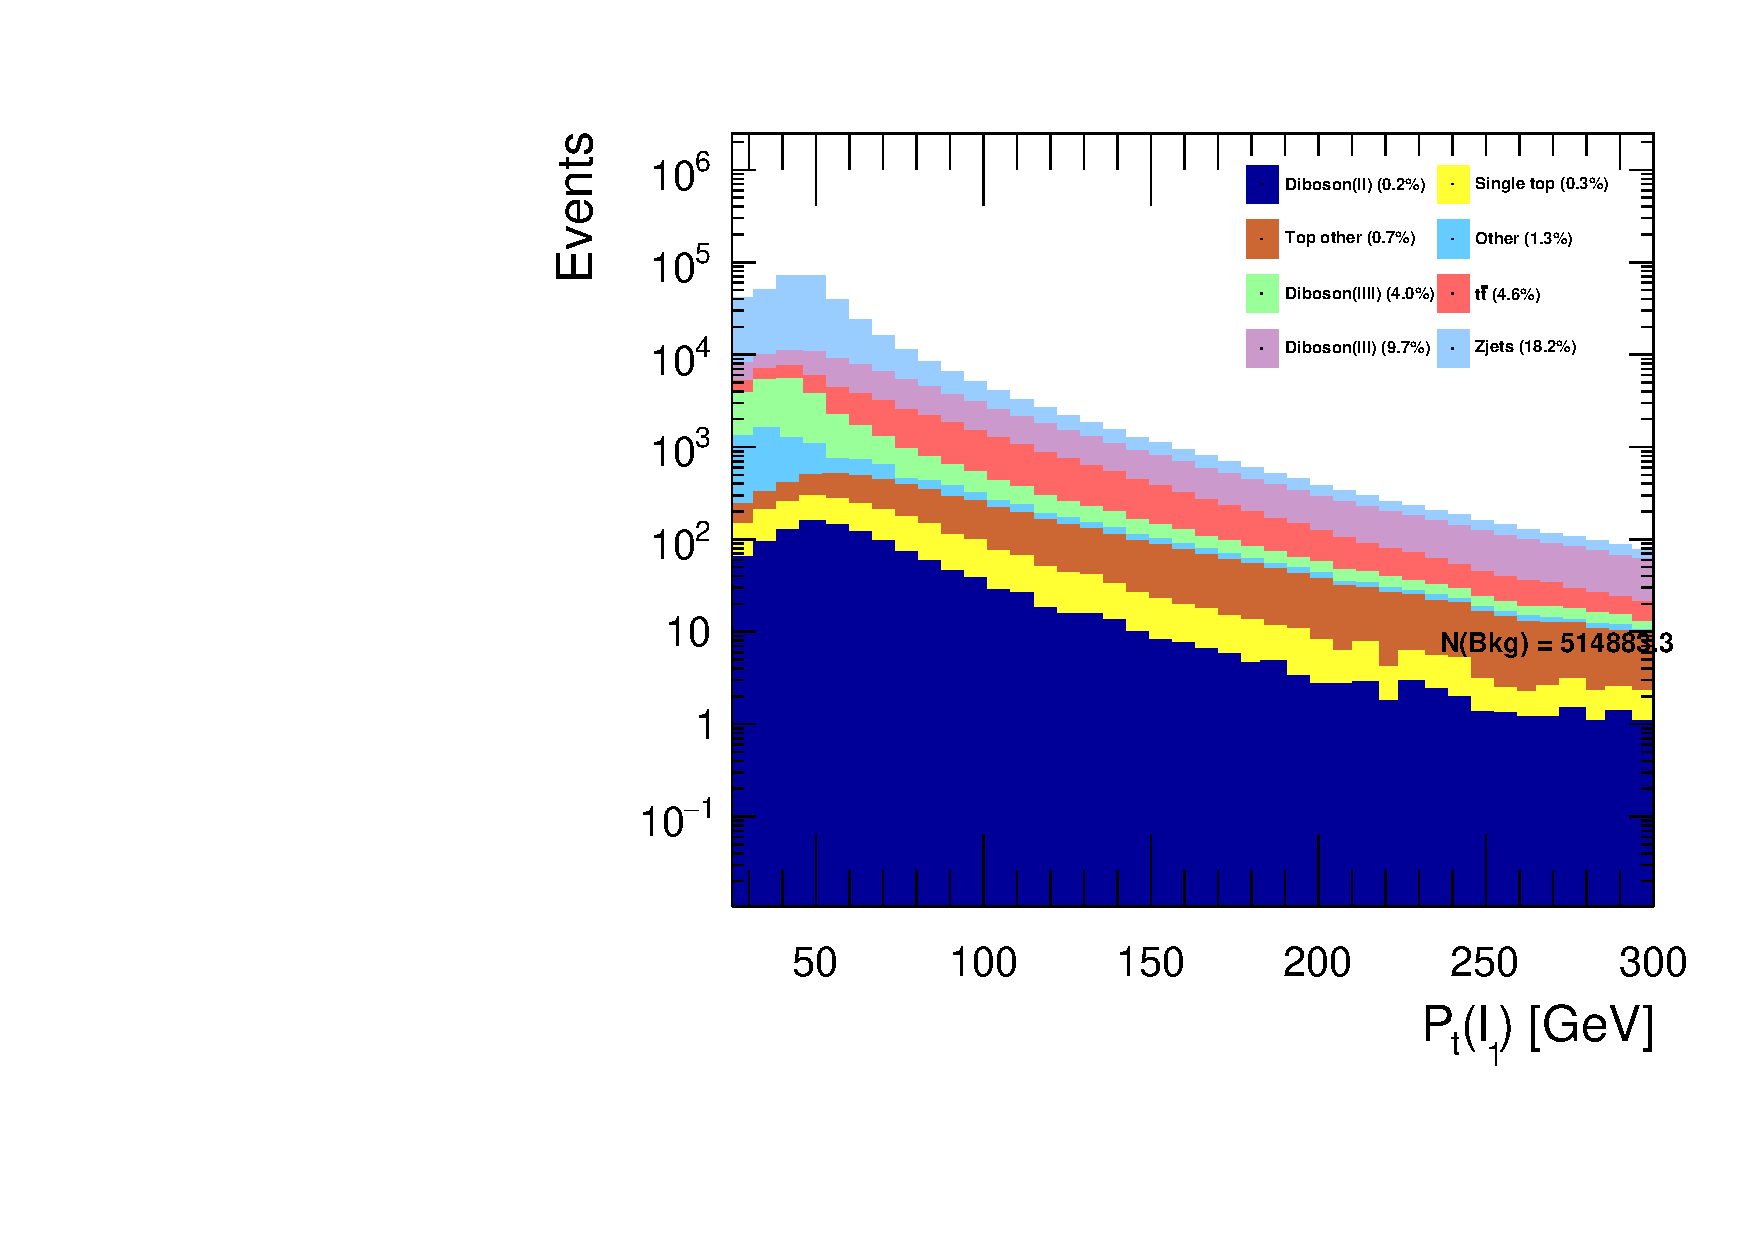
\includegraphics[width=\textwidth]{Figures/FeaturesHistograms/lep1_Pt_nNeg.pdf}
        \vspace{-.75cm}
        \caption{}
        \label{fig:lep1_Pt_nNeg}
    \end{subfigure}
    }
    \makebox[0.95\linewidth][c]{%
    \centering
    \begin{subfigure}{.525\textwidth}
        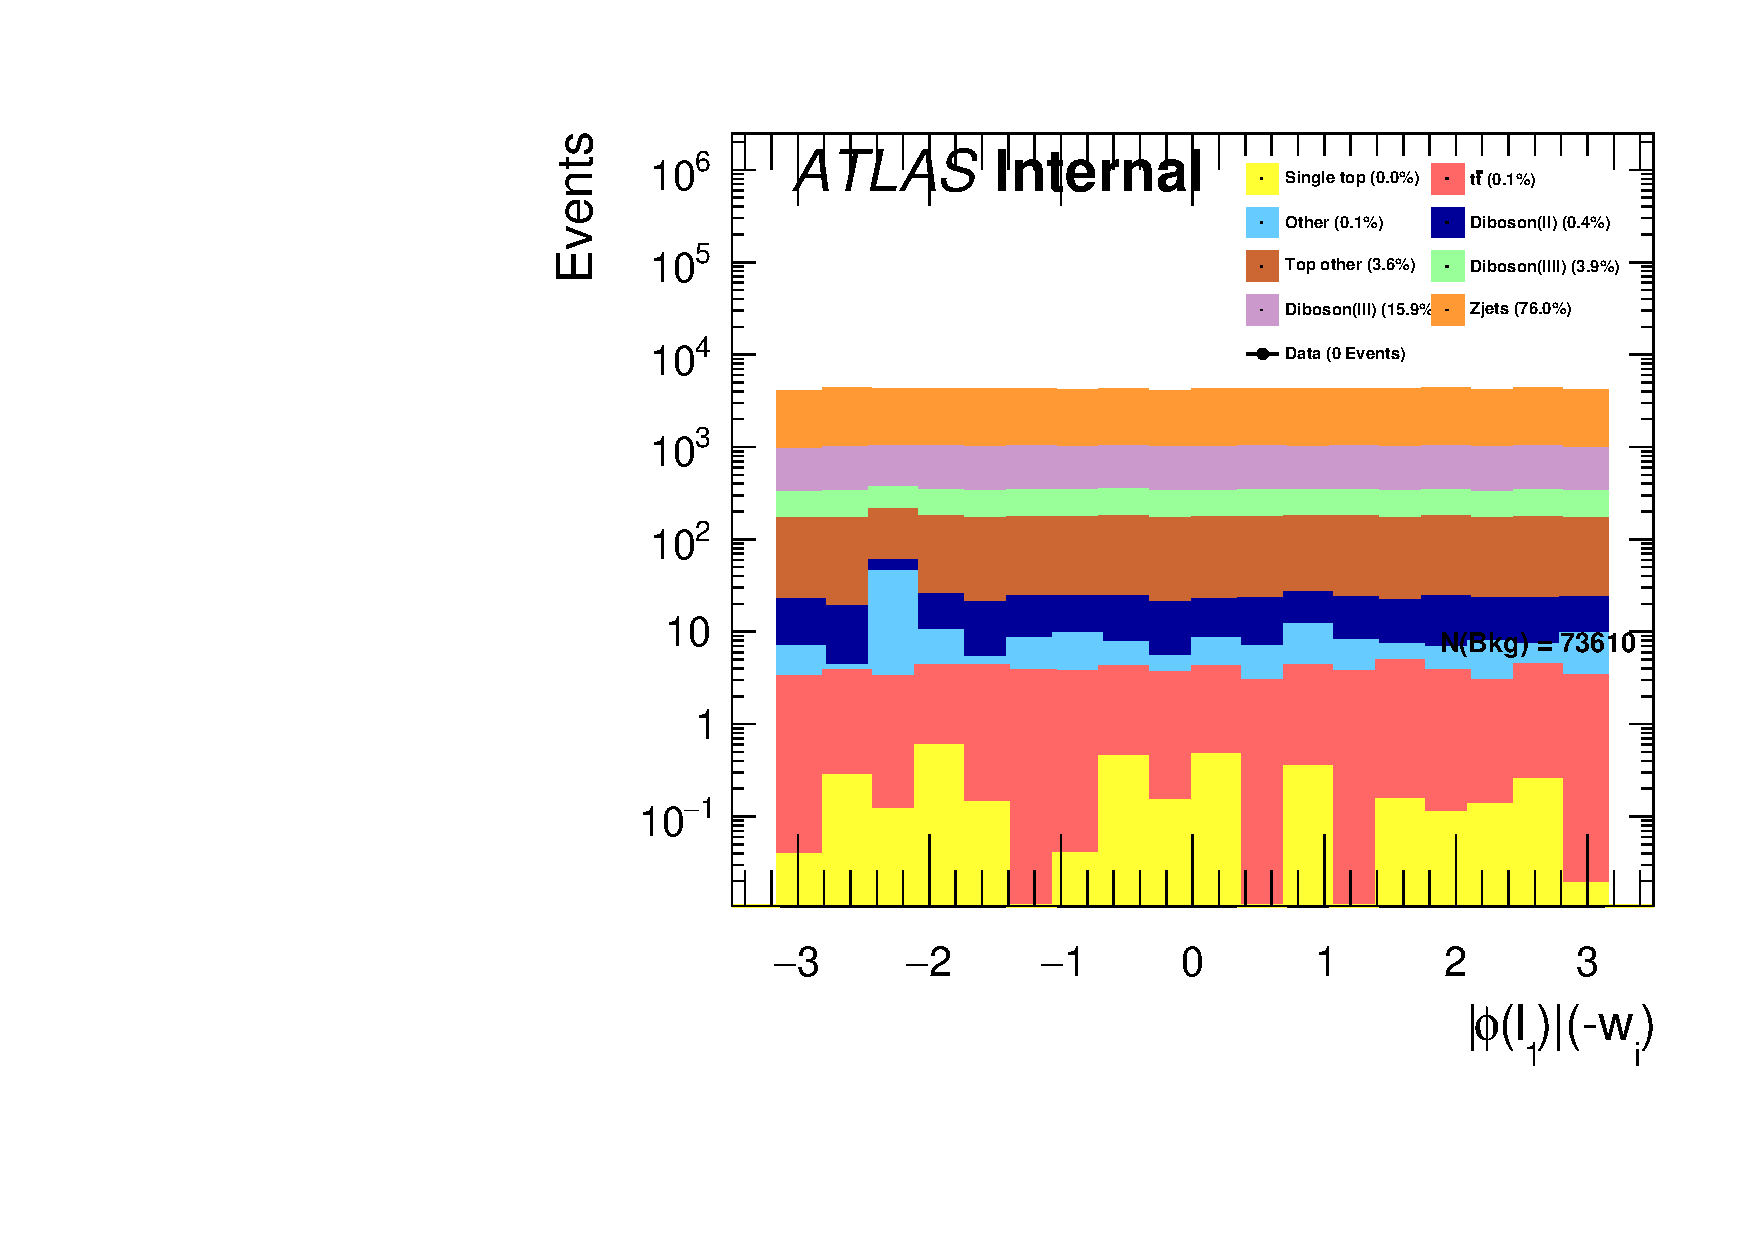
\includegraphics[width=\textwidth]{Figures/FeaturesHistograms/lep1_Phi_Neg.pdf}
        \vspace{-.75cm}
        \caption{}
        \label{fig:lep1_Phi_Neg}
    \end{subfigure}
    \begin{subfigure}{.525\textwidth}
        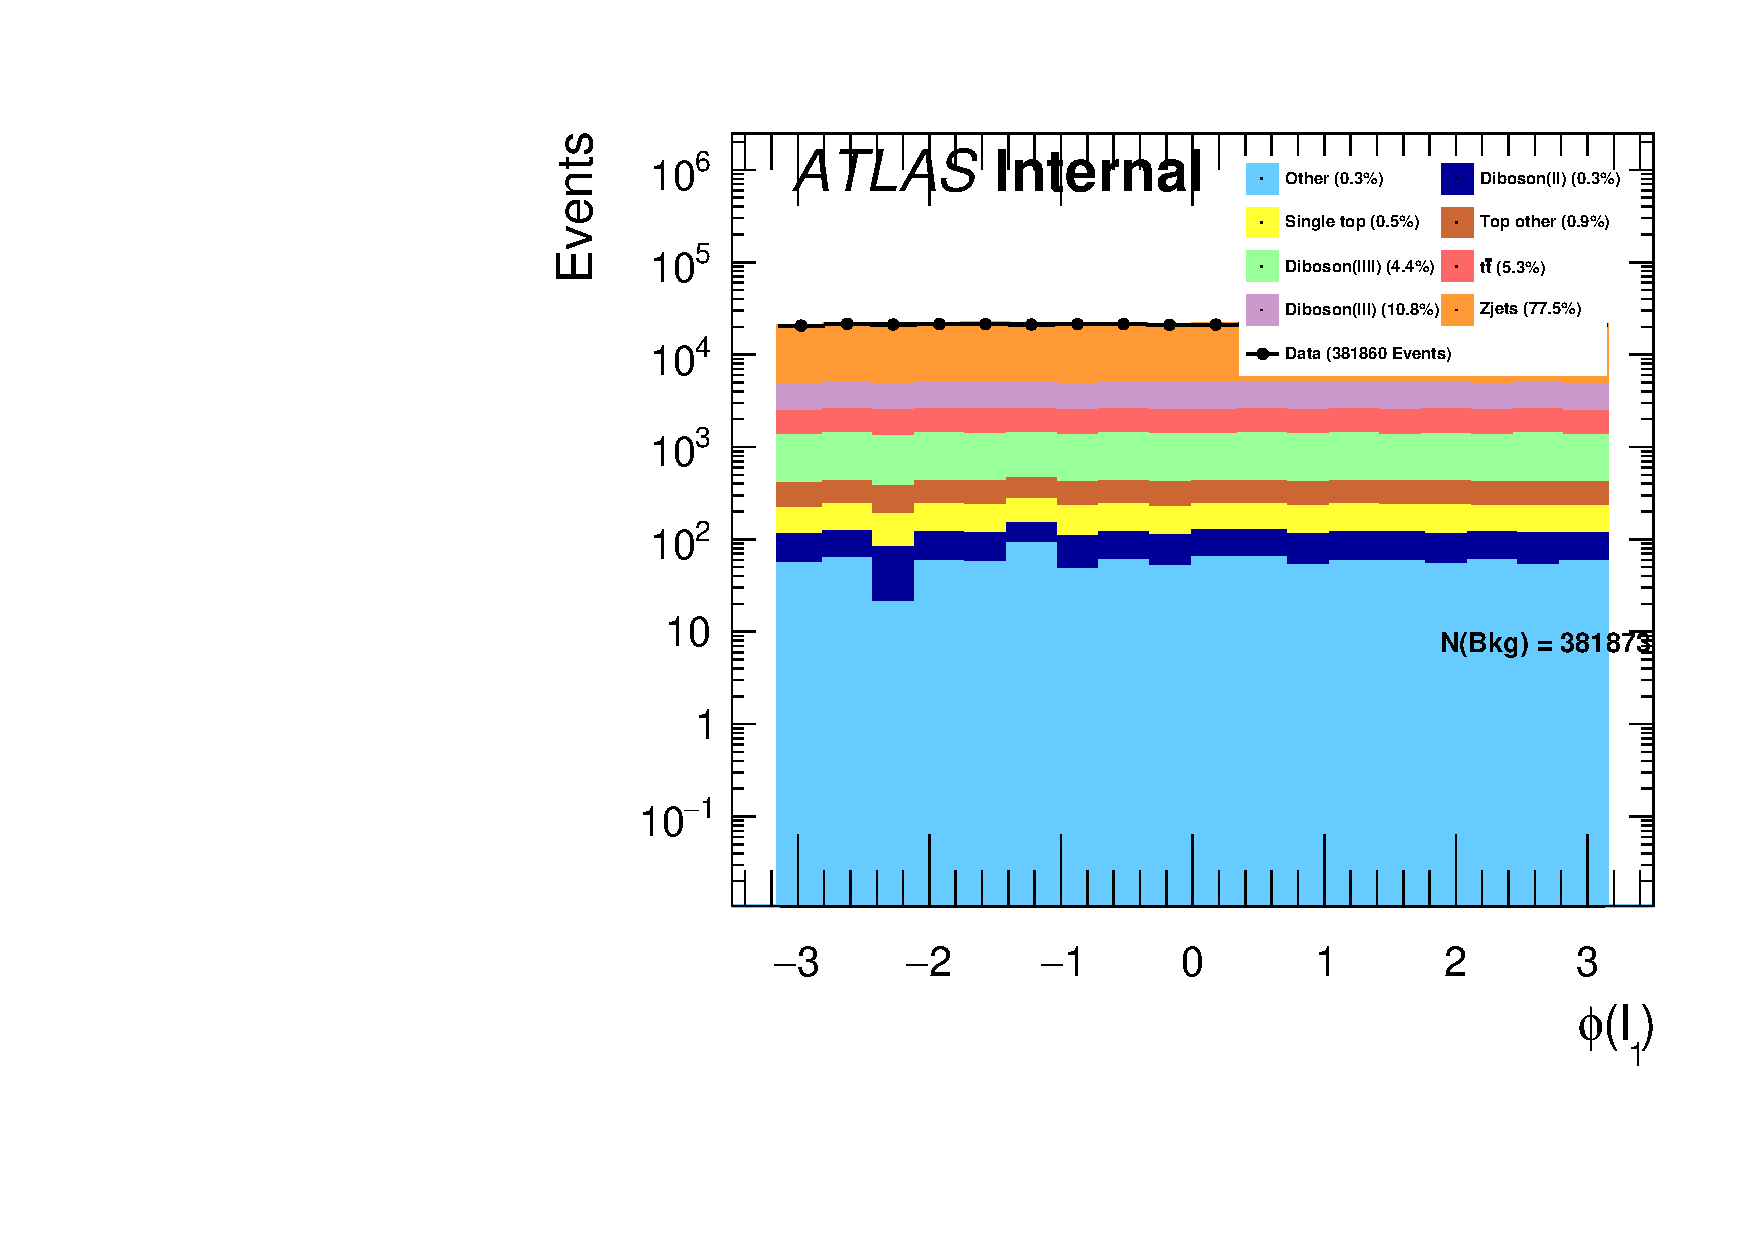
\includegraphics[width=\textwidth]{Figures/FeaturesHistograms/lep1_Phi_nNeg.pdf}
        \vspace{-.75cm}
        \caption{}
        \label{fig:lep1_Phi_nNeg}
    \end{subfigure}
    }
    \caption[The event distributions of the leading lepton for the features $P_t$ and $\phi$, for events with negative 
    weights and all events.]{The event distributions of the leading lepton for the features $P_t$ and $\phi$. 
    Figures \ref{fig:lep1_Pt_Neg} and \ref{fig:lep1_Phi_Neg} display only the events with 
    negative weights (for $P_t$ and $\phi$ respectively) whereas \ref{fig:lep1_Pt_nNeg} 
    and \ref{fig:lep1_Phi_nNeg} show the full data set.}
\end{figure}
How one chooses to deal with this problem can heavily effect results and many solutions 
are suggested as a consequence. Given the main focus of this rapport, the 
simplest solution was chosen. The solution was motivated by the internal notes of 
the \ac{ATLAS} article \cite{Aad:2800889}, who introduced the solution when faced with the same 
problem. The solution is to take the absolute value and normalize all the weights, conserving 
the total sum of the weights and at the same time changing all negative signs. The simple procedure 
is shown bellow in equation \ref{eq:negw},
\begin{align}\label{eq:negw}
    w_i & = P \mid w_i \mid\,  \\
    P  & =  \sum_{j=0}^{N-1}\frac{ w_j}{\mid w_j \mid},
\end{align}
where $w_i$ is the weight of an event i, $i \in [0,N-1]$ and N equals the total number of events.
\section{Defining the Signal Region and Calculating the Significance}
When producing an output, I define the signal region through a brute force method which maximizes the significance. 
Based on trial and error and the study of the output from several models, I found that due to the unbalanced ratio of 
signal to background, a successful signal region would have to be very 'strict'. Therefore, for each model output I implemented a 
set of 200 cuts ranging from $0.9$ to the highest output of the model, with most cuts falling in the range of $>0.98$. For each cut
the significance is calculated where all signal and background events larger than said cut are included in the signal region. The cut 
corresponding to the largest significance, is used to define the final signal region.  
\\
In most calculations of the significance I use equations \ref{eq:Z1}. This equation does not include any 
uncertainty, which is why any results using said equation is only for comparison reasons between the different \ac{ML}
models. In the final sections of the thesis, I am interested in including uncertainty in the results. To do this I utilize 
a function in ROOT, the \emph{RooStats.NumberCountingUtils.BinomialExpZ}, which takes the number of expected signal and background, 
as well as the systematic uncertainty of the background.